\section{Desenvolvimento}

% ------ estrutura
\subsection{Ferramentas Utilizadas}
    \begin{frame}\frametitle{Ferramentas Utilizadas}
        % ide, g++, make, gui builder
        \begin{itemize}
            \item IDE: NetBeans 7.1.1 e Eclipse 3.7.2
            \item Outros programas: g++, make, vim
            \item 
        \end{itemize}
    \end{frame}
    
\subsection{Ferramentas Desenvolvidas}
    \begin{frame}\frametitle{Ferramentas Desenvolvidas}
        \begin{itemize}
            \item Operam sobre vídeos no formato bruto (YUV).
            \item Stand-alone.
            \item Acessadas através da \emph{interface} gráfica.
        \end{itemize}
        \begin{itemize}
            \item \emph{raffle}: gerador de arquivos de degradação.
            \item \emph{block}: efeito de blocagem.
            \item \emph{blur}: efeito de borramento.
            \item \emph{metric}: avaliador objetivo.
            \item \emph{NetSim}: simulador de perda de pacotes em um \emph{streaming}.
        \end{itemize}
    \end{frame}
    
    \begin{frame}\frametitle{Raffle}
        \begin{itemize}
            \item Gerador de arquivos de degradação organizados em colunas.
            \item Valor conforme distribuição: constante, uniforme, normal ou triangular.
        \end{itemize}
        \\ ~\\
        ./raffle -e 30 -o out.rff -u uniform -r 1,5 -d uniform -p 0,60 -d triangular -p 0,40,30
        \begin{table}[!h]
            \centering
            \caption{Exemplo de execução do raffle.}
            \label{tab:rafflerun}
            \begin{tabular}{|c|c|c|c|c|c|}
                \hline
                21 21 & 19 32 & 22 27 & 31 29 & 17 32 & 49 34 \\
                42 14 & 20 32 & 23 27 & 32 29 & 23 16 &  0 35 \\
                43 14 & 10 25 & 26  2 &  9 17 & 24 16 &  1 35 \\
                 0 16 & 11 25 & 29 29 & 10 17 & 25 16 & 35 18 \\
                18 32 & 12 25 & 30 29 & 11 17 & 26 16 & 36 18 \\
                \hline
            \end{tabular}
        \end{table}
    \end{frame}

    \begin{frame}\frametitle{Block}
        Gerador de efeito de blocagem. Parâmetros:
        \begin{table}[!h]
	        \begin{tabular}{ll}
	            \texttt{-i}  & vídeo original. \\
	            \texttt{-o}  & vídeo degradado. \\
	            \texttt{-r}  & arquivo\_raffle (2 colunas). \\
	            \texttt{-s}  & dimensões do vídeo de entrada no formato WxH \\ 
	            & (largura por altura em \emph{pixels}). \\
	            \texttt{-w}  & tamanho da janela da DCT. \\
	            \texttt{-l}  & níveis DCT à serem eliminados, separados por vírgulas. \\
	            \texttt{-h}  & menu de ajuda. \\
            \end{tabular}
        \end{table}
    \end{frame}
    
    \begin{frame}\frametitle{Blur}
        Gerador de efeito de borramento. Parâmetros:
        \begin{table}[!h]
	        \begin{tabular}{ll}
	            \texttt{-i}  & vídeo original. \\
	            \texttt{-o}  & vídeo degradado. \\
	            \texttt{-r}  & arquivo\_raffle (2 colunas). \\
	            \texttt{-s}  & dimensões do vídeo de entrada no formato WxH \\ 
	            & (largura por altura em \emph{pixels}). \\
	            \texttt{-b}  & tipo do filtro a ser aplicado. \\
	            \texttt{-w}  & tamanho do filtro. \\
	            \texttt{-h}  & menu de ajuda. \\
	        \end{tabular}
        \end{table}
    \end{frame}
    
    \begin{frame}\frametitle{NetSim}
        Simualdor de rede. Parâmetros:
        \begin{table}[!h]
	        \begin{tabular}{ll}
	            \texttt{-i}  & vídeo original. \\
	            \texttt{-o}  & vídeo degradado. \\
	            \texttt{-t}  & (opcional) Se presente, a entidade de descarte considerada \\
	            & é um TS, caso contrário a unidade é um pacote UDP. \\
	            \texttt{-r}  & arquivo\_raffle (2 colunas). \\
	        \end{tabular}
        \end{table}
    \end{frame}
    
    \begin{frame}\frametitle{Metric}
        Realiza avaliações objetivas segundo as métricas MSE, PSNR e MSSIM.
        \begin{table}[!h]
	        \begin{tabular}{ll}
	            \texttt{-i}  & vídeo a ser comparado. \\
	            \texttt{-r}  & vídeo de referência. \\
	            \texttt{-s}  & dimensões dos vídeos no formato WxH. \\ 
	            & (largura por altura em \emph{pixels}). \\
	            \texttt{-m}  & métrica desejada: MSE, PSNR ou MSSIM. \\
	            \texttt{-w}  & tamanho da janela (apenas para métrica MSSIM). \\
	        \end{tabular}
        \end{table}
    \end{frame}

\subsection{Interface Gráfica}
        \begin{frame}\frametitle{Sessão}
            Permite a configuração e execução de uma sessão, segundo as métricas DSIS e SDSCE.
		    \begin{figure}
			    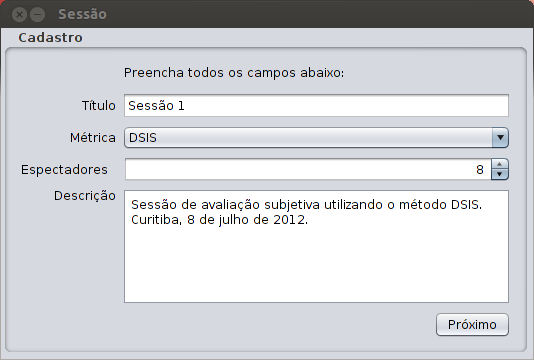
\includegraphics[width=0.6\textwidth]{./imgs/sessao1.png}
			    \caption{Tela de criação de nova sessão.}
			    \tiny
			    Fonte: Autoria própria.
		    \end{figure}
        \end{frame}
        
        \begin{frame}\frametitle{Ferramentas e Utilidades}
            Permite visualizar arquivos de degradação (extensão .rff) e vídeos.
		    \begin{figure}
			    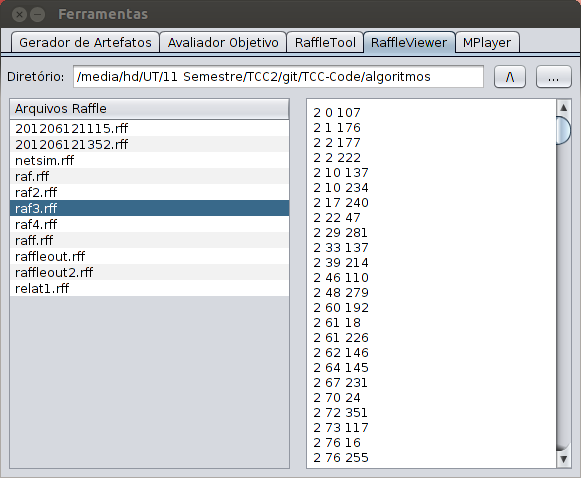
\includegraphics[width=0.6\textwidth]{./imgs/ferramentas-viewer.png}
			    \caption{Utilidades.}
			    \tiny
			    Fonte: Autoria própria.
		    \end{figure}
        \end{frame}
        
        \begin{frame}\frametitle{Gerador de Artefatos}
            Permite gerar vídeos degradados no formato YUV.
		    \begin{figure}
			    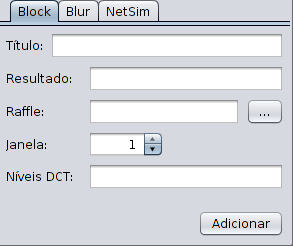
\includegraphics[width=0.6\textwidth]{./imgs/ferramentas-gerador.png}
			    \caption{Parte da tela do gerador de artefatos.}
			    \tiny
			    Fonte: Autoria própria.
		    \end{figure}
        \end{frame}
        
        \begin{frame}\frametitle{Avaliador Objetivo}
            Permite realizar avaliações objetivas.
		    \begin{figure}
			    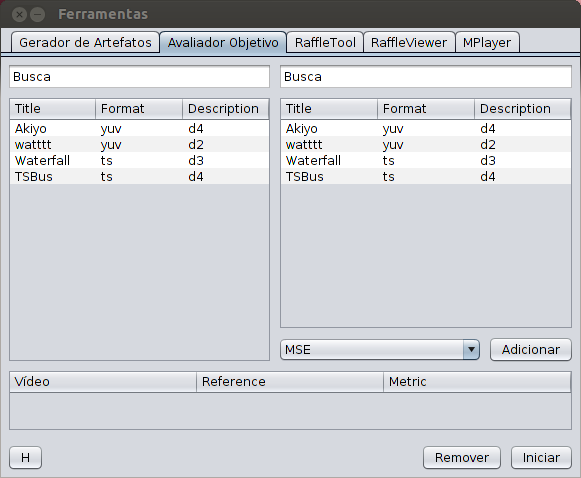
\includegraphics[width=0.6\textwidth]{./imgs/ferramentas-avaliador.png}
			    \caption{Tela do avaliador objetivo.}
			    \tiny
			    Fonte: Autoria própria.
		    \end{figure}
        \end{frame}
        
        \begin{frame}\frametitle{Gerador de Arquivos de Degradação}
		    \begin{figure}
			    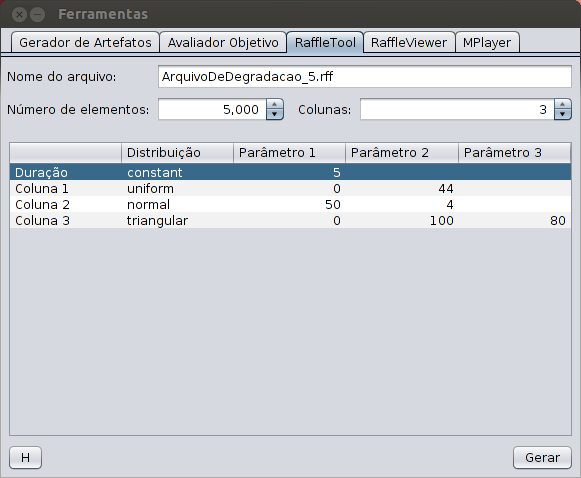
\includegraphics[width=0.6\textwidth]{./imgs/ferramentas-raffle.png}
			    \caption{Tela do gerador de arquivos de degradação.}
			    \tiny
			    Fonte: Autoria própria.
		    \end{figure}
        \end{frame}
